\documentclass[../main/main.tex]{subfiles}
\graphicspath{{./figures/}}

\makeatletter
\renewcommand{\@chapapp}{Travaux pratiques -- TP}
\makeatother

\toggletrue{student}
\HideSolutionstrue

\begin{document}
\setcounter{chapter}{0}

\chapter{D\'etermination de focales de lentilles}

\ifstudent{
	\begin{prgm}
		\begin{tcb}*(ror)"how"{Savoir-faire}
			\begin{itemize}[label=$\diamond$, leftmargin=10pt]
				\item Former une image.
				\item Éclairer un objet de manière adaptée.
				\item Modéliser expérimentalement à l'aide de plusieurs lentilles un
				      dispositif optique d'utilisation courante.
				\item Optimiser la qualité d'une image (alignement, limitation des
				      aberrations).
				\item Estimer une valeur approchée d’une distance focale.
			\end{itemize}
		\end{tcb}
	\end{prgm}

	\section{Objectifs}

	\begin{itemize}[label=$\diamond$, leftmargin=10pt]
		\item Réaliser des alignements sur un banc optique~;
		\item Reconnaître rapidement une lentille convergente et une lentille
		      divergente~;
		\item Déterminer une distance focale par différentes méthodes.
	\end{itemize}

	\section{S'approprier}

	Trois méthodes sont possibles pour la détermination expérimentale de la distance
	focale d'une lentille convergente.

	\subsection{Méthode de \textsc{Bessel}}

	La méthode de \textsc{Bessel} utilise le montage ci-dessous où $D$, la distance
	objet-écran, est fixée, avec $D>4f'$.
	\begin{figure}[]
		\centering
		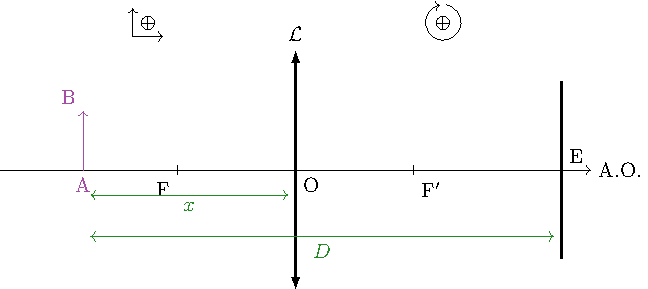
\includegraphics[width=.8\linewidth]{lent_conv-condition_plain}
	\end{figure}

	La méthode de \textsc{Bessel} pour déterminer la distance focale $f'$ consiste donc à
	imposer une distance $D$ entre un objet et un écran et à rechercher les deux
	positions de la lentille $\Lc$ qui donnent une image nette de l'objet sur l'écran
	$E$. En mesurant les deux distances $D$ et $d$ (distance entre les deux
	positions de la lentille pour lesquelles on obtient une image nette), on peut
	calculer la valeur de la distance focale image $f'$ de la lentille.

	\subsection{Méthode de \textsc{Silbermann}}

	La méthode de Silberman est le cas particulier de la méthode de \textsc{Bessel} pour
	lequel $D=4f'$.

	\subsection{Utilisation de la relation de conjugaison}

	Cette méthode consiste à utiliser une régression linéaire permettant de vérifier
	la relation de conjugaison~:

	\[
		\frac{1}{\OAp}-\dfrac{1}{\OA} = \dfrac{1}{f'}
	\]
}

\setcounter{section}{2}
\section{Analyser}

\subsection{Méthode de \textsc{Bessel}}
\label{ssec:bessel}
\ifstudent{
	\begin{minipage}{0.49\linewidth}
		À l'aide d'une lentille mince convergente $\Lc$ de distance focale image
		$f'$, on veut former l'image d'un objet réel sur un écran situé à une
		distance $D$ de l'objet. En déplaçant la lentille, on trouve une ou deux
		positions O$_1$ et O$_2$ qui donnent une image nette sur l'écran (cf.\ figure
		ci-contre).
	\end{minipage}
	\hfill
	\begin{minipage}{0.49\linewidth}
		\begin{center}
			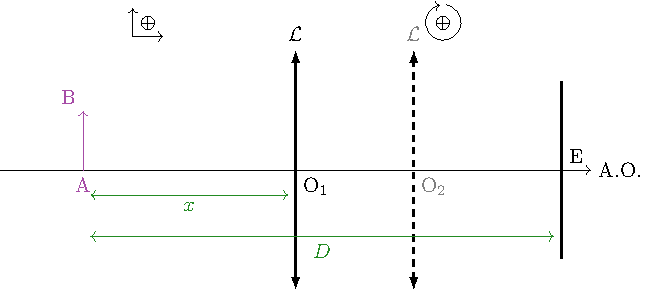
\includegraphics[width=0.9\textwidth]{lent_conv-condition_bessel}
		\end{center}
	\end{minipage}
}

\begin{enumerate}[label=\clenumi]
	\item \switch{
		      Déterminer dans ce cas, les deux expressions des positions
		      correspondantes de la lentille notées $x_1=\obar{\rm O_1A}$ et
		      $x_2=\obar{\rm O_2A}$ en fonction de $D$ et $f'$ et vérifier que
		      celles-ci n'existent que si $D>4f'$.
	      }{
		      ~
		      \smallbreak
		      \begin{isd}
			      Avec les notations de l'énoncé, la relation de Descartes devient
			      \begin{align*}
				      \frac{1}{f'}                 & = \frac{1}{D-x} - \frac{1}{-x} \\
				      \Leftrightarrow \frac{1}{f'} & = \frac{x + D-x}{x(D-x)}       \\
				      \Leftrightarrow f'           & = \frac{x(D-x)}{D}             \\
				      \Leftrightarrow 0            & = x^2 - xD + f'D
			      \end{align*}
			      Ce trinôme du second degré a pour discriminant
			      \[
				      \boxed{\Delta = D^2-4f'D = D(D-4f')}
			      \]
			      \tcblower
			      $x$ étant une distance physique, on cherche $\Delta \geq 0$.
			      \begin{itemize}[label=$\diamond$, leftmargin=10pt]
				      \item $\Delta = 0$ si $D = 4f'$, et alors
				            \[
					            \boxed{x = \frac{D}{2}}
				            \]
				      \item $\Delta > 0$ si $D > 4f'$, et alors
				            \[
					            \boxed{x_\pm = \frac{D\pm\sqrt{D(D-4f')}}{2}}
				            \]
			      \end{itemize}
		      \end{isd}
	      }
	\item \switch{
	      Exprimer $d=\obar{\rm O_1O_2}$ , puis montrer qu'alors
	      \centers{$\boxed{f'=\dfrac{D^2-d^2}{4D}}$}
	      }{
	      Ainsi, la zone de netteté de l'image se situe entre $x_+$ et $x_-$, et a
	      donc une largeur
	      \[
		      \boxed{d = x_+ - x_- = \sqrt{D(D-4f')}}
		      \Lra
		      \boxed{f' = \frac{D^{2}-d^{2}}{4D}}
	      \]
	      }
	\item \switch{
		      À l'aide du TP00 - mesures et incertitudes, déterminer analytiquement
		      l'expression de l'incertitude-type sur $f'$ en fonction de $d$, $D$, $u(d)$
		      et $u(D)$. Il faut pour cela déterminer l'incertitude d'une fraction avec
		      IV/A), l'incertitude sur $d^{2}/4D$ avec IV/B) produit de puissances, et
		      enfin l'incertitude sur $f'$ avec IV/B) somme ou différence.
	      }{
		      Soit $d$, $D$ les valeurs mesurées. Pour calculer l'incertitude d'une
		      fraction, par exemple $u(D/4)$, on utilise
		      \[
			      u \left( \frac{D}{4} \right) = \abs{\frac{D/4}{D}}u(D)
			      \Lra
			      u \left( \frac{D}{4} \right) = \frac{u(D)}{4}
		      \]
		      Ensuite,
		      \begin{align*}
			      u \left( \frac{d^{2}}{4D} \right)                & =
			      \frac{u \left( \frac{d^{2}}{D} \right)}{4}
			      \\\qet
			      \frac{u \left( d^{2}D^{-1} \right)}{d^{2}D^{-1}} & =
			      \sqrt{2 \left( \frac{u(d)}{d} \right)^{2} +
				      1 \left( \frac{u(D)}{D} \right)^{2}}
			      \\\Ra
			      u \left( \frac{d^{2}}{4D} \right)                & = \frac{d^{2}}{4D}
			      \sqrt{2 \left( \frac{u(d)}{d} \right)^{2} +
				      1 \left( \frac{u(D)}{D} \right)^{2}}
		      \end{align*}
		      Finalement,
		      \begin{align*}
			      u \left( f' \right)         & =
			      \sqrt{u \left( \frac{D}{4} \right)^{2} +
				      u \left( \frac{d^{2}}{4D} \right)^{2}}
			      \\
			                                  & =
			      \frac{1}{4} \sqrt{
				      \left( \frac{u(D)}{D} \right)^{2} +
				      \left( \frac{d^{2}}{D} \right)^{2}
				      \left[
					      2 \left( \frac{u(d)}{d} \right)^{2} +
					      \left( \frac{u(D)}{D} \right)^{2}
					      \right]
			      }
			      \\\Lra
			      \Aboxed{u \left( f' \right) & =
				      \frac{1}{4} \sqrt{
					      u(d)^{2}\times 2 \frac{d^{2}}{D^{2}} +
					      u(D)^{2} \left[ 1 + \frac{d^{4}}{D^{4}} \right]
				      }
			      }
		      \end{align*}
	      }
	\item \switch{
		      Déterminer un protocole expérimental permettant la mesure d'une
		      distance focale par cette méthode.
	      }{
		      On place la lentille convergente sur le banc optique, avec l'objet le plus
		      près de la lampe source pour maximiser son éclairement et l'écran fixé à une
		      distance $D \approx \SI{50}{cm}$ de l'objet.
		      \smallbreak
		      On cherche une première position de la lentille telle que l'image soit nette
		      sur l'écran. On mesure distance objet-lentille $x_1$. On déplace la lentille
		      jusqu'à ce qu'on retrouve une image nette, et on mesure $x_2$.
		      \smallbreak
		      On calcule $d = x_2-x_1$ et on calcule $f'$.
	      }
\end{enumerate}

\subsection{Méthode de \textsc{Silbermann}}

\begin{enumerate}[label=\clenumi, start=5]
	\item \switch{
		      Montrer qu'il existe un cas particulier intéressant où $x_1=x_2$.
	      }{
		      Déjà fait en \ref{ssec:bessel}
	      }
	\item \switch{
		      En déduire la nouvelle expression de $f'$ dans ce cas.
	      }{
		      Avec la relation de conjugaison, on trouve aisément
		      \[
			      \boxed{f' = \frac{D}{4}}
		      \]
	      }
	\item \switch{
		      Déterminer un protocole expérimental permettant d'utiliser cette
		      deuxième méthode.
	      }{
		      Avec le même montage que précédemment, on place l'écran loin de la lentille.
		      On déplace la lentille pour trouver les deux positions de netteté. Si on en
		      distingue effectivement deux, on rapproche l'écran, et on recherche une
		      nouvelle fois les positions.
		      \smallbreak
		      Procéder ainsi jusqu'à ce qu'il n'y ait plus qu'une position pour laquelle
		      l'image est nette. On aura alors $f' = D/4$.
	      }
\end{enumerate}

\subsection{Méthode utilisant la relation de conjugaison}

\begin{enumerate}[label=\clenumi, start=8]
	\item \switch{
		      Déterminer un protocole expérimental permettant d'utiliser cette troisième
		      méthode. Vous l'expliciterez clairement et me le proposerez avant mise en
		      application.
	      }{
		      Avec la même lentille, on prend une distance aléatoire OA et on déplace
		      l'écran pour avoir une image nette. On mesure OA'.
		      \smallbreak
		      On répète l'expérience pour environ 10 mesures. On tracera ensuite
		      \[
			      y = ax + b
			      \qav
			      \left\{
			      \begin{array}{rcl}
				      y & = & \frac{1}{\OAp}
				      \\
				      a & = & -1
				      \\
				      x & = & \frac{1}{\OA}
				      \\
				      b & = & \frac{1}{f'}
			      \end{array}
			      \right.
		      \]
		      On pourra forcer $a = -1$, et on cherchera l'ordonnée à l'origine pour avoir
		      $1/f'$~: ainsi, on aura $f' = 1/b$.
	      }
\end{enumerate}

\section{Réaliser}
\ifstudent{
	\subsection{Matériel disponible}

	\begin{isd}
		\begin{itemize}[label=$\diamond$, leftmargin=10pt]
			\item Lentilles convergentes et divergentes (en dioptries, $\delta$)~: -10~;
			      -3~; -2~; -1~; 1~; 2~; 3~; 8~; 10.
			\item Lampe spectrale et écran dépoli
			\item Banc d'optique et supports
		\end{itemize}
		\tcblower
		\begin{itemize}[label=$\diamond$, leftmargin=10pt]
			\item Support magnétique constitué des lettres $F$ et de la mini-règle
			\item Écran
			\item Réglet
		\end{itemize}
	\end{isd}

	\subsection{Reconnaissance rapide convergente ou divergente}

	\begin{tcb}[cnt](impo){Attention}
		Afin de se protéger de la lumière émise par la lampe, insérer un écran
		dépoli entre la lampe et l'objet.
	\end{tcb}

	Avec les lentilles disponibles, vérifier expérimentalement les critères suivants
	après les avoir expliqués de manière théorique à l'aide de tracés de rayons~:

	\begin{enumerate}
		\item \textbf{Observation directe}~: Les lentilles convergentes sont des
		      lentilles à bords minces, les lentilles divergentes sont à bords épais.
		\item \textbf{Effet loupe}~: Une lentille convergente donne d'un objet placé
		      à faible distance une image virtuelle, droite et agrandie.
		\item \textbf{Effet anti-loupe}~: Une lentille divergente donne d'un objet
		      réel proche ou éloigné une image virtuelle, droite et réduite.
		\item \textbf{Déplacement transversal}~: Lorsqu'on déplace transversalement
		      une lentille convergente devant un objet placé à faible distance, son
		      image se déplace dans le sens inverse de celui de la lentille. Dans le
		      cas d'une lentille divergente, le sens du déplacement est identique.
	\end{enumerate}

	\subsection{Projection sur un écran avec une lentille convergente}

	\begin{enumerate}
		\item Réaliser un alignement sur le banc d'optique permettant de projeter
		      l'image d'un objet sur un écran à l'aide d'une lentille convergente.
		\item Pour une position de la lentille donnée, déterminer le grandissement
		      $\gamma=\dfrac{\ABp}{\AB}$ et vérifier la relation~:
		      \[
			      \gamma=\dfrac{\OAp}{\OA}
		      \]
		      en mesurant $\OAp$ et $\OA$ à l'aide d'un réglet.
	\end{enumerate}
}
\setcounter{subsection}{3}
\subsection{Mesure précise de la distance focale d'une lentille convergente}

\begin{enumerate}[label=\sqenumi, start=9]
	\item \switch{
		      Mettre en œuvre les trois méthodes proposées dans les parties Analyser
		      et S'approprier pour déterminer la distance focale de la lentille
		      convergente notée ($+10$). Vous noterez les valeurs expérimentales,
		      calculs et résultats sur le \textit{notebook} \texttt{Capytale}
		      correspondant\ftn{\url{https://capytale2.ac-paris.fr/web/c/1228-1802331}}
		      et les résultats sur vos copies.
		      \smallbreak
	      }{
		      On trouve~:
		      \subsubsection{\textsc{Bessel}}
		      \textit{En cours…}
		      \subsubsection{\textsc{Silbermann}}
		      \textit{En cours…}
		      \subsubsection{\textsc{régression}}
		      \textit{En cours…}
	      }
	\item \switch{
		      Comparer alors les résultats obtenus par les différentes méthodes.
		      Vous calculerez dans chaque cas l'écart relatif par rapport à la
		      valeur théorique.
	      }{
	      }
\end{enumerate}

\section{Valider et conclure}

\switch{
	\begin{enumerate}[label=\sqenumi, start=11]
		\item Déterminer l'incertitude-type sur la détermination de la distance focale $f'$
		      obtenue dans le cas de la méthode de \textsc{Bessel}. On évaluera dans un
		      premier temps l'incertitude de type B sur la détermination de $D$ et $d$ (avec
		      incertitude composée de type différence) puis on calculera l'incertitude-type
		      sur $f'$ dont l'expression a été trouvée dans la partie Analyser.
		      \smallbreak
		      Calculer alors l'écart normalisé. Conclure.
		\item Faites de même par méthode de \textsc{Monte-Carlo}, sur l'activité
		      \texttt{Capytale}.
	\end{enumerate}
}{
}

\end{document}
